\chapter{进阶}

第2章中客户端与服务器端的例子演示了在Java中进行Socket编程的基本模式,下一步我们将介绍如何把这些基本概念应用到各种编程模型中去,如多任务处理、非阻塞式I/O、
广播等。 

\section{多任务处理} 

	我们在第2章中所介绍的基本TCP响应服务器一次只能处理一个客户端的请求。当一个客户端向一个已经被其他客户端占用的服务器发送连接请求时,虽然其在连接建立后即可向服务器端发送数据,服务器端在处理完已有客户端的请求前,却不会对新的客户端作出响应,。这种类型的服务器称为"迭代服务器(iterative server)"。迭代服务器按顺序处理客户端的请求,也就是说在完成了对前一客户端的服务后,才会对下一个客户端进行响应。这种服务器最适用于每个客户端所请求的连接时间都被限制在较小范围内的应用中,而对于允许客户端请求长时间服务的情况,后续客户端将面临无法接受的长时间等待。 

	为了更直观地说明这种情况,我们在TCPEchoClient.java文件中调用Socket构造器的代码段后面加入Thread.sleep()方法来实现10秒的暂停,并实验多个客户端同时访问TCP响应服务器的情况。 这里的sleep调用是用来模拟一个客户端长时间占用服务器的情况,如慢速的文件或网络I/O(输入输出)。通过实验可以看到,一个新的客户端必须等到服务器对前面所有已连接的客户端完成服务后,才能获得服务器的对它的请求的响应。 

	我们需要一种方法可以独立处理每一个连接,并使它们不会产生相互干扰,而Java的多线程技术刚好满足了这一需求,这一机制使服务器能够方便地同时处理多个客户端的请求。通过使用多线程,一个应用程序可以并行执行多项任务,就好像有多个Java虚拟机在同时运行。(实际上是多个线程共享了同一个Java虚拟机。)在我们的响应服务器中,可以为每个客户端分配一个执行线程来实现。到目前为止,我们所看到的全部例子都是由一个简单执行main()方法的单线程组成的。 

	本节我们将介绍两种实现并行服务器(concurrent servers)的编程方法,分别为:一客户一线程(thread-per-client),即为每一个客户端连接创建一个新的线程;线程池(thread pool),即将客户端连接分配给一组事先创建好的线程。我们还会对Java中能够简化实现多线程服务器的内置工具进行描述。 

	\subsection{Java 多线程}

		Java提供了两种在一个新线程中执行任务的方法:1)为Thread类定义一个带有run()方法的子类,在run()方法中包含要执行的任务,并实例化这个子类;或2)定义一个实现了Runnable接口的类,并在run()方法中包含要执行的任务,再将这个类的一个实例传递给Thread的构造函数。无论哪种情况,新线程创建后并不立即执行,而是要等到其start()方法被调用。第一种方法只适用于没有继承于其他类的类,因此我们专注于第二种方法,它能够适用于多种情况。Runnable接口中只包含一个方法原型: 

		\begin{verbatim}
		interface Runnable { void run(); } 
		\end{verbatim}

		当Thread对象的start()方法被调用时,Java虚拟机将在一个新的线程中执行该对象的run()方法,从而实现与其他任务并行执行。同时,原来的线程从调用start()方法的地方返回,继续独立执行。(值得注意到是,直接调用run()方法并不产生新线程,而只会像其它类方法一样在调用者线程中执行)由于每个线程的run()方法是以任意的方式交错声明的,因此无法准确预测各个线程的执行顺序。

		在下面的例子中,ThreadExample.java实现了Runnable接口,并在run()方法中反复向系统输出流打印一句问候语。 

		\lstinputlisting[language=Java,firstline=1]{src/ch04/ThreadExample.java}

		1.实现Runnable接口的声明:

		ThreadExample实现了Runnable接口,因此可以将其传递给Thread类的构造函数。如果ThreadExample没有提供run()方法,编译器将会给出警告。 

		2.类成员变量与构造函数:

		每个ThreadExample类的实例都包含了自己的问候语句,存放在类实例的字符串成员变量中。 

		3.run()方法:

		循环语句将反复执行以下内容: 

		打印出线程名和当前实例问候语句:

		静态方法Thread.currentThread()将从调用它的线程中返回一个该线程的引用,getName()方法返回一个包含该线程名单字符串。 

		暂停线程:

		每个线程实例在打印出问候信息后,都将随机暂停一定的时间(在0至100毫秒之间),这通过把暂停的毫秒数作为参数传递给Thread.sleep()静态方法来实现。Math.random()方法返回0.0到1.0之间的一个double型随机数。Thread.sleep()方法可以被其他线程打断,并抛出InterruptedException异常。本例中没有包含打断该方法的调用,因此这个应用中不会发生这种异常。 

		4.main()方法:

		main()方法中的三行声明都完成了如下工作:

		1)用不同的问候语字符串创建了ThreadExample类的一个新实例,

		2)将这个新实例传递给Thread类的构造函数,

		3)调用新的Thread实例的start()方法。在主线程已经结束时,每个线程正在独立地执行ThreadExample类的run()方法。注意,Java虚拟机只有在所有非守护线程(见Thread API)都执行完毕的情况下才终止。 

		在程序运行的时候,三条问候语句将交错地打印到控制台中。很多因素都会对线程真实的执行顺序产生影响,而这些因素是用户无法观察到的。对于我们例子中的这种服务器端,每个客户端的执行过程都与其他客户端相互独立,这就非常适合使用多线程技术来实现。但是,如果客户端的执行过程涉及到需要更新服务器端线程间的共享信息,这将变得相当麻烦。在这种情况下,必须非常小心,以确保不同的线程间在共享数据上得到了妥善的同步,否则,会导致共享信息不一致的状况发生,更麻烦的是这些问题追踪起来还非常困难。如果要完整地介绍并发技术和工具需要一整本书的篇幅,例如Goetz等人就写了一本非常好的著作。 

	\subsection{服务器协议}

		既然我们将要介绍的多任务服务器方法与特定的客户端-服务器协议相互独立,我们希望能够实现一个同时满足两者的协议。EchoProtocol中给出了回显协议的代码。这个类的静态方法handleEchoClient()中封装了对每个客户端的处理过程。除添加了写日志功能(马上会对其介绍)外,这段代码与TCPEchoServer.java中的连接处理部分几乎完全一致。该方法的参数是客户端Socket实例和Logger实例的引用。 

		EchoProtocol类实现了Runnable接口(run()方法只是根据该实例的Socket和Logger引用,简单地调用handleEchoClient()方法),因此我们可以创建一个独立执行run()方法的线程。另外,服务器端的协议执行过程可以通过直接调用这个静态方法实现(为其传入Socket和Logger实例的引用)。 

		\lstinputlisting[language=Java,firstline=1]{src/ch04/EchoProtocol.java}

		1.声明实现Runnable接口:

		2.类成员变量和构造函数:

		每个EchoProtocol实例都包含了一个相应连接的套接字和对logger实例的引用。 

		3.handleEchoClient():

		实现回显协议: 

		从套接字中获取输入/输出流:

		接收和回显:

		循环执行直到连接关闭(由read()方法返回值为-1指示),每次循环中在接收到数据后就立即写回。 

		在日志中记录连续的详细信息: 

		同时记录远端的SocketAddress和回显的字节数。 

		异常处理:

		将异常写入日志。 

		你的服务器每分钟将执行上千次客户端请求。现在有用户报告了一个问题。那么如何才能确定到底发生了什么呢?是不是服务器的问题呢?也许是客户端在破坏这个协议。为了处理这种情况,大部分的服务器都将它们的活动记录写入日志。这里我们只对写日志作非常基础的介绍,不过,你得知道还存在更多的日志记录功能以满足企业级需求。 

		首先我们介绍Logger类,它代表了本地或远端的一个日志记录工具。通过该类的一个实例,我们就可以记录服务器的各种活动信息,就像在EchoProtocol中演示的那样。或许你会在服务器上使用多个日志记录器(logger),每个记录器以不同的方式负责不同的需求。例如,你可以有不同的日志记录器分别负责记录操作、安全和出错消息。在Java中,每个日志记录器由一个全局唯一的名字识别。按照如下代码调用Logger.getLogger()静态工厂方法即可获取一个Logger实例: 

		\begin{verbatim}
			Logger logger = Logger.getLogger("practical"); 
		\end{verbatim}

		这行代码用于获取名字为"practical"的记录器。如果这个名字的记录器不存在,则用这个名字创建一个新的记录器,否则,返回已存在的记录器实例。无论在程序中获取名字为"practical"的记录器多少次,都将返回同一个实例。 

		有了日志记录器,需要记录什么内容呢?这取决于你要做什么。如果服务器在正常地运行,你可能不想将服务器执行的每一步都记录到日志中,因为记录日志是要消耗系统资源的,如为日志项分配存储空间,写日志需要占用服务器的处理时间等。另一方面,如果是为了调试,你可能就希望记录服务器执行的每一步。为了对不同情况进行处理,记录器中通常包含了日志项的等级或严格度的概念。Level类中就封装了消息的重要程度信息。每个Logger实例都有一个当前等级,每条日志消息也有对应的等级,低于Logger实例的当前等级的消息将被抛弃(即不写入日志)。每个等级都有一个对应的整数值,因此等级之间可以相互比较和排序。系统识别的Level实例共有7种,同时还能创建用户定义的等级,不过通常没有必要这样做。内置的等级(定义为Level类的静态字段)包括:severe,warning,info,config,fine,finer,和finest。 

		当你写日志的时候,消息又去哪儿呢?记录器将消息发送到一个或多个Handler实例中,该实例用来发布这些消息。默认情况,每个logger有一个ConsoleHandler用来将消息打印到System.err中。你也可以为一个logger改变或添加handler(如FileHandler)。注意,与logger一样,每个handler也有自己的最小日志等级,因此要发布一条消息,它的等级必须同时高于logger和handler的等级阈值。logger和handler的可配置性很高,包括他们的最小等级。 

		Logger对我们来说一个重要的特征是它是线程安全的(thread-safe),即可以在并行运行的不同线程中调用它的方法,而不需要在调用者中添加额外的同步措施。如果没有这个特征,由不同线程记录的不同消息将错乱无章地写到日志中。 

		Logger: 查找/创建 

		\lstinputlisting[language=Java,firstline=1,lastline=2]{src/ch04/ThreadExample.txt}

		这些静态工厂方法返回指定名字的Logger实例,必要时创建新的实例。 

		一旦有了logger,我就需要做的就是……写日志。Logger提供了从细粒度到粗粒度的日志记录工具,并能够区分消息的不同等级甚至消息的上下文。 

		Logger: 记录日志消息 

		\lstinputlisting[language=Java,firstline=11,lastline=26]{src/ch04/ThreadExample.txt}

		severe(),warning()等方法根据其名字对应等级,将给定的符合等级的消息写入日志。entering() 和exiting() 方法在程序进入或退出给定类的指定方法时将记录写入日志。注意你也可以选择性地指定额外信息,如参数和返回值等。throwing()方法用于将指定方法所抛出的异常信息写入日志。log()方法提供了一种一般性的日志记录方式,该方法可以指定需要记录的消息等级和内容,并可以选择性地添加异常信息。当然还存在很多其他记录日志的方法,这里我们只提到了主要的几种。 

		我们可能希望能够通过设置最小记录等级或日志消息处理器的等级,来定制自己的记录器。 

		Logger: 设置/获取日志的等级和处理器 

		\lstinputlisting[language=Java,firstline=31,lastline=37]{src/ch04/ThreadExample.txt}

		getHandlers()方法返回一个包含了和该记录器关联的所有日志处理器数组。addHandler()和removeHandler()方法用于给该记录器添加或删除日志处理器。getLevel()和setLevel()方法用于获取和设置日志记录的最小等级。isLoggable()方法则在该记录器能够记录所给定的等级 的日志时返回true。 

		现在我们准备介绍一些不同的方法来实现并行服务器。 

	\subsection{一客户一线程} 

		在一客户一线程(thread-per-client)的服务器中,为每个连接都创建了一个新的线程来处理。服务器循环执行一些任务,在指定端口上侦听连接,反复接收客户端传入的连接请求,并为每个连接创建一个新的线程来对其进行处理。 

		TCPEchoServerThread.java实现了这种一客户一线程的服务器结构。它与迭代服务器非常相似,也是用一个循环来接收和处理客户端的请求。主要不同点在于这种服务器为每个连接创建了一个新的线程来处理,而不是直接处理。(这是可行的,因为EchoProtocol类实现了Runnable接口。)因此,当多个客户端几乎同时连接服务器时,后请求的客户端不需要等服务器对前面的客户端处理结束后才获得服务,相反,它们看起来是同时接受的服务(虽然比对单一客户端进行服务要稍微慢一些)。 

		\lstinputlisting[language=Java,firstline=1]{src/ch04/TCPEchoServerThread.java}

		1.参数解析和服务器套接字/日志记录器创建:

		2.一直反复循环,处理传入的连接请求:

		接收传入的连接请求:

		创建一个新的Thread实例来处理新的连接:

		由于EchoProtocol类实现了Runnable接口,所有我们可以将其新实例作为参数传递给Thread类的构造函数,当调用Thread的start()方法时,新线程将执行EchoProtocol的run()方法(run()方法里面调用的是handleEchoClient()方法)。 

		为连接开始执行新的线程并记录日志:第25-26行 

		Thread类的getName()方法返回一个包含新线程名字的String实例。 

	\subsection{线程池} 

		每个新线程都会消耗系统资源:创建一个线程将占用CPU周期,而且每个线程都自己的数据结构(如,栈)也要消耗系统内存。另外,当一个线程阻塞(block)时,JVM将保存其状态,选择另外一个线程运行,并在上下文转换(context switch)时恢复阻塞线程的状态。随着线程数的增加,线程将消耗越来越多的系统资源。这将最终导致系统花费更多的时间来处理上下文转换和线程管理,更少的时间来对连接进行服务。那种情况下,加入一个额外的线程实际上可能增加客户端总服务时间。 

		我们可以通过限制总线程数并重复使用线程来避免这个问题。与为每个连接创建一个新的线程不同,服务器在启动时创建一个由固定数量线程组成的线程池(thread pool)。当一个新的客户端连接请求传入服务器,它将交给线程池中的一个线程处理。当该线程处理完这个客户端后,又返回线程池,并为下一次请求处理做好准备。如果连接请求到达服务器时,线程池中的所有线程都已经被占用,它们则在一个队列中等待,直到有空闲的线程可用。 

		与一客户一线程服务器一样,线程池服务器首先创建一个ServerSocket实例。然后创建N个线程,每个线程都反复循环,从(共享的)ServerSocket实例接收客户端连接。当多个线程同时调用同一个ServerSocket实例的accept()方法时,它们都将阻塞等待,直到一个新的连接成功建立。然后系统选择一个线程,新建立的连接对应的Socket实例则只在选中的线程中返回。其他线程则继续阻塞,直到成功建立下一个连接和选中另一个幸运的线程。 

		行为就像是一组迭代服务器。与一客户一线程服务器不同,线程池中的线程在完成对一个客户端的服务后并不终止,相反,它又重新开始在accept()方法上阻塞等待。TCPEchoServerPool.java中演示了一个线程池的例子。 

		\lstinputlisting[language=Java,firstline=1]{src/ch04/TCPEchoServerPool.java}

		1.设置:

		要侦听的端口号和线程的数量都作为参数传递给main()。对参数进行解析后再创建ServerSocket 和Logger实例。注意要它们都必须声明为常量(final),因为它们将在下面创建的匿名类中引用。 

		2.创建并启动threadPoolSize个新线程:

		循环的每一次迭代都会创建一个继承于Thread的匿名类的实例。当调用该实例的start()方法时,这个线程就会执行该匿名类的run()方法。run()方法将反复循环,接受客户端的连接请求,并传递给EchoProtocol进行处理。 

		接受连接请求:

		由于有N个不同线程在执行同一个循环,那么最多有N个线程在servSock的accept()方法上阻塞等待传入的连接请求。对于任何一个连接,系统保证了只要一个线程能够获得其对应的Socket。在一个客户端连接被创建时,如果没有线程在accept()方法上阻塞等待(即,所有线程都在忙着为其他连接服务),系统则将新的连接排列在一个队列中,直到下一次调用accept()方法(见第6.4.1节)。 

		将客户端套接字传递给EchoProtocol.handleEchoClient()方法:

		handleEchoClient()方法中封装了协议的详细内容。该方法在连接处理完成后将相关信息写入日志,处理过程中遇到的异常也将写入日志。 

		处理accept()方法抛出的异常:

		由于线程的重复使用,线程池的方法只需要付出创建N次线程的系统开销,而与客户端连接总数无关。由于可以控制最大并发执行线程数,我们就可以控制线程的调度和资源开销。当然,如果我们创建的线程太少,客户端还是有可能等很长时间才获得服务,因此,线程池的大小需要根据负载情况进行调整,以使客户端连接的时间最短。理想的情况是有一个调度工具,可以在系统负载增加时扩展线程池的大小(低于大小上限),负载较轻时缩减线程池的大小。Java恰好就有这种工具,我们将在下一节进行介绍。 

	\subsection{系统管理调度:Executor接口}

		在上一节中我们已经看到,将客户服务器协议的细节封装起来(如EchoProtocol.java),就可以通过同一个协议实现来使用不同的"调度"方法(如,TCPEchoServerThread.java和TCPEchoServerThreadPool.java)。实际上,对于调度方法本身来说也是这样。Executor接口(java.util.concurrent包的一部分)就代表了一个根据某种策略来执行Runnable实例的对象,其中可能包括了排队和调度的细节,或如何选择要执行的任务。Executor接口只定义了一个方法: 

		\begin{verbatim}
			interface Executor { void execute(Runnable task); } 
		\end{verbatim}

		Java提供了大量的内置Executor接口实现,它们都可以简单方便地使用,也可以进行扩展性的配置。其中一些还提供了处理维护线程等繁琐细节的功能。例如,如果一个线程因为未捕获的异常或其他故障停止,它们就自动创建一个新的线程来替换原来的线程。 

		ExecutorService接口继承于Executor接口,并提供了一个更高级的工具来关闭服务器,包括正常的关闭和突然的关闭。ExecutorService还允许在完成任务后返回一个结果,这需要用到Callable接口,它和Runnable接口很像,只是多了一个返回值。 

		我们可以通过调用Executors类的各种静态工厂方法来获取ExecutorService实例。示例程序TCPEchoServerExecutor.java演示了基本Executor工具的使用方法。 

		\lstinputlisting[language=Java,firstline=1]{src/ch04/TCPEchoServerExecutor.java}

		1.设置:

		端口号是唯一的参数。与前面的例子一样,我们要创建ServerSocket实例和Logger实例。这里它们不必声明为常量,因为我们不需要用匿名的Thread子类。 

		2.获取一个Executor实例:

		Executors类的newCachedThreadPool()静态工厂方法创建了一个ExecutorService实例。在使用一个实现了Runnable接口的实例调用它的execute()方法时,如果必要它将创建一个新的线程来处理任务。然而,它首先会尝试使用已有的线程。如果一个线程空闲了60秒以上,则将移出线程池。这个策略几乎总是比前面两个TCPEchoServer*例子的效率高。 

		3.反复循环,接收并执行连接:

		当一个新的连接请求到来时,将创建一个新的EchoProtocol实例并传递给service的execute()方法,该方法要么将其分配给一个已有的线程,要么创建一个新的线程来处理它。值得注意的是,当达到稳定状态时,缓存线程池服务最终将保持合适的线程数,以使每个线程都保持忙碌,同时又很少创建或销毁线程。 

		只要有一个设计为使用Executor来调度客户端的服务器,我们就可以通过简单地改变Executor实例的类型来实现不同的调度策略。例如,如果我们想使用像TCPEchoServerPool.java中那样的固定大小的线程池,只需要改变与设置调度服务相关的一行代码: 

		\lstinputlisting[language=Java,firstline=41,lastline=41]{src/ch04/ThreadExample.txt}

		我们可以将线程池的大小设为1,转换成使用单一线程处理所有的客户端连接,或者使用以下方法来实现: 

		\lstinputlisting[language=Java,firstline=42,lastline=42]{src/ch04/ThreadExample.txt}

		在Executor方法中,如果一个"工人"线程由于某些故障死掉了,Executor将创建一个新的线程来代替它。而且,任务是在Executor的内部排队,而不是像我们最初的服务器那样在网络系统中排队。到现在为止,我们仅仅触及到了Java并发包的表层功能而已。 

\section{阻塞和超时}

	Socket的I/O调用可能会因为多种原因而阻塞。数据输入方法read()和receive()在没有数据可读时会阻塞。TCP套接字的write()方法在没有足够的空间缓存传输的数据时可能阻塞。 ServerSocket的accept()方法和Socket的构造函数都会阻塞等待,直到连接建立(见第6.4节)。同时,长的信息往返时间,高错误率的连接和慢速的(或已发生故障的)服务器,都可能导致需要很长的时间来建立连接。所有这些情况,只有在连接请求得到满足后这些方法才会返回。当然,调用一个已经阻塞的方法将使应用程序停止(并使运行它的线程无效)。 

	当程序在等待一次调用的完成时如果还有其他任务要执行的情况会怎样(如,更新"忙碌"状态的光标或响应用户请求)?这些程序可能没有时间来等待一个阻塞的方法调用。那UDP数据报文丢失的情况呢?如果我们阻塞等待接收一个数据报文,而它已经丢失,则会导致程序无限期地阻塞下去。这里,我们将对各种阻塞方法和限制阻塞的途径进行探讨。在第5章,我们将接触到NIO包中的更加强大的非阻塞工具。 

	\subsection{accept(),read()和receive()} 

		对于这些方法,我们可以使用Socket类、ServerSocket类和DatagramSocket类的setSoTimeout()方法,设置其阻塞的最长时间(以毫秒为单位)。如果在指定时间内这些方法没有返回,则将抛出一个InterruptedIOException异常。对于Socket实例,在调用read()方法前,我们还可以使用该套接字的InputStream的available()方法来检测是否有可读的数据。 

	\subsection{连接和写数据}

		Socket类的构造函数会尝试根据参数中指定的主机和端口来建立连接,并阻塞等待,直到连接成功建立或发生了系统定义的超时。不幸的是,系统定义的超时时间很长,而Java又没有提供任何缩短它的方法。要改变这种情况,可以使用Socket类的无参数构造函数,它返回的是一个没有建立连接的Socket实例。需要建立连接时,调用该实例的connect()方法,并指定一个远程终端和超时时间(毫秒)。 

		write()方法调用也会阻塞等待,直到最后一个字节成功写入到了TCP实现的本地缓存中。如果可用的缓存空间比要写入的数据小,在write()方法调用返回前,必须把一些数据成功传输到连接的另一端(详情见第6.1节)。因此,write()方法的阻塞总时间最终还是取决于接收端的应用程序。不幸的是Java现在还没有提供任何使write()超时或由其他线程将其打断的方法。所以如果一个可以在Socket实例上发送大量数据的协议可能会无限期地阻塞下去。(第6.2节介绍了这个特点可能导致的灾难性后果) 

	\subsection{限制每个客户端的时间}

		现在假设要实现一个为每个客户端限定了服务时间的回显协议。也就是说我们定义一个了目标,TIMELIMIT,并在协议中实现经过TIMELIMIT毫秒后,实例就自动终止。协议实例保持了对剩余服务时间的跟踪,并使用setSoTimeout()方法来保证read()方法的阻塞时间不会超过TIMELIMIT。由于没有办法限制write()调用的时间,我们并不能保证所定义的时间限制真正有效。尽管如此,TimelimitEchoProtocol.java还是实现了这种方法;要与TCPEchoServerExecutor.java一起使用,只需要简单地将while循环的第二行改为: 

		\lstinputlisting[language=Java,firstline=51,lastline=51]{src/ch04/ThreadExample.txt}

		第5章将介绍更强大的机制(在所有的I/O调用上,包括写操作)来限制线程阻塞时间,这些机制都使用NIO包的工具类实现。 

		\lstinputlisting[language=Java,firstline=1]{src/ch04/TimelimitEchoProtocol.java}

		TimelimitEchoProtocol类与EchoProtocol类非常相似,唯一的区别在于它试图将回显连接的总服务时间限制在10秒钟之内。当handleEchoClient() 方法被调用时,就通过当前时间和服务期限计算出了服务的截止时间。每次read()调用结束后将重新计算当前时间与截止时间的差值,即剩余服务时间,并将套接字超时设置为该剩余时间。 

\section{多接收者}

	到目前为止,我们的套接字都处理的是两个实体之间的通信,通常是一个服务器和一个客户端。这种一对一的通信方法有时称为单播(unicast)。而对于某些信息,多个接收者都可能对其感兴趣。对于这种情况,我们可以向每个接收者单播一个数据副本,但是这样做效率可能非常低。由于将同样的数据发送了多次,在一个网络连接上单播同一数据的多个副本非常浪费带宽。实际上,如果我们想要以固定频率发送数据,网络连接带宽就已经限制了其所能支持的接收者数量。例如,如果我们的视频服务器以1Mbps的速率发送数据流,而其网络连接速率是3Mbps(良好的连接速率),那么该连接最多只能同时支持3个用户。 

	幸运的是网络提供了一个更有效地使用带宽的方法。我们可以将复制数据包的工作交给网络来做,而不是由发送者负责。在我们的视频服务器例子中,我们将数据流的单个副本通过服务器连接发送到网络,再由网络在适当的时候将数据复制成多份。使用这种复制模式,无论有多少客户端,服务器都只需要使用其网络连接的1Mbps带宽。 

	有两种类型的一对多(one-to-many)服务:广播(broadcast)和多播(multicast)。对于广播,(本地)网络中的所有主机都会接收到一份数据副本。对于多播,消息只是发送给一个多播地址(multicast address),网络只是将数据分发给那些表示想要接收发送到该多播
	地址的数据的主机。总的来说,只要UDP套接字允许广播或多播。 

	\subsection{广播} 

		广播UDP数据报文与单播数据报文相似,唯一的区别是其使用的是一个广播地址而不是一个常规的(单播)IP地址。注意,IPv6并没有明确地提供广播地址;然而,有一个特殊的全节点(all - nodes)、本地连接范围(link-local-scope)的多播地址,FFO2::1,发送给该地址的消息将多播到一个连接上的所有节点。IPv4的本地广播地址(255.255.255.255)将消息发送到在同一广播网络上的每个主机。本地广播信息决不会被路由器转发。在以太网上的一个主机可以向在同一以太网内的其他主机发送消息,但是该消息不会被路由器转发。IPv4还指定了定向广播地址,允许向指定网络中的所有主机进行广播;然而,由于互联网上的大部分路由器都不转发定向广播消息,我们在此不对其进行介绍。 

		并不存在可以向网络范围内所有主机发送消息的广播地址。至于为什么没有,请考虑向互联网上每台主机发送广播消息可能产生的影响。在这种地址发送单个数据报文就可能会由路由器产生非常大量的数据包副本,并可能会耗尽所有网络的带宽。误用(恶意的或意外的)该地址的后果会非常严重,因此IP协议的设计者故意没有定义互联网范围的广播机制。 

		即使如此,本地广播功能还是非常有用的,它通常用于在网络游戏中处于同一本地(广播)网络的玩家之间交换状态信息。在Java中,单播和广播的代码是相同的。要实现具有广播功能的应用程序,我们可以简单地在VoteClientUDP.java中使用广播目的地址。不过这里有个问题,你能发现它吗?提示:广播不能使用连接。像以前那样运行VoteServerUDP.java程序(你还可以同时运行多个接收者)。注意:有些操作系统不允许普通用户进行广播操作,在这种系统上程序将无法正常运行。 

	\subsection{多播} 

		与广播一样,多播与单播之间的一个主要区别是地址的形式。一个多播地址指示了一组接收者。IP协议的设计者为多播分配了一定范围的地址空间,IPv4中的多播地址范围是224.0.0.0到239.255.255.255,IPv6中的多播地址是任何由FF开头的地址。除了少数系统保留的多播地址外,发送者可以向以上范围内的任何地址发送数据。Java中多播应用程序主要通过MulticastSocke实例进行通信,它是DatagramSocket的一个子类。重点需要理解的是,一个MulticastSocket实例实际上就是一个UDP套接字(DatagramSocket),其包含了一些额外的可以控制的多播特定属性。我们的下一个例子实现了投票信息的多播发送者和接收者。 

		\lstinputlisting[language=Java,firstline=1]{src/ch04/VoteMulticastSender.java}

		我们的单播发送者和多播发送者仅有的重要区别是:

		1)对给定地址是否是多播地址进行了验证,

		2)为多播数据报文设置了初始的TTL值(生命周期, Time To Live)。每个IP数据报文中都包含了一个TTL,它被初始化为某个默认值,并在每个路由器转发该报文时递减(通常是减1)。当TTL值减为0时,就丢弃该数据报文。通过设置TTL的初始值,我们可以限制数据包从发送者开始所能传递到的最远距离。实际上多播情况下一个TTL=4的数据包并不一定从开始跳足4跳,但一定不能超过4跳。

		与广播不同,网络多播只将消息副本发送给指定的一组接收者。这组接收者叫做多播组(multicast group),通过共享的多播(组)地址确定。接收者需要一种机制来通知网络它对发送到某一特定地址的消息感兴趣,以使网络将数据包转发给它。这种通知机制叫做加入一组(joining a group),可以由MulticastSocket类的joinGroup()方法实现。我们的多播接收者加入了一个特定的组,接收并打印该组的一条多播消息,然后退出。 

		\lstinputlisting[language=Java,firstline=1]{src/ch04/VoteMulticastReceiver.java}

		我们的多播和单播接收者唯一的重要区别是,多播接收者表明希望从哪个多播地址接收数据来加入多播组。本书的网站上还有另一个多播发送者和接收者的例子。MulticastImageSender.java将一组由命令行参数指定的图片(JPEG或GIF)以3秒的时间间隔传输。MulticastImageReceiver.java则接收每一个图片并在窗口中显示。 

		多播数据报文实际上可以通过DatagramSocket中发送,只需要简单地指定一个多播地址。不过MulticastSocket还有一些DatagramSocket没有的能力,包括1)允许指定数据报文的TTL,和2)允许指定和改变通过哪个接口将数据报文发送到组(接口由其互联网地址确定)。另一方面,一个多播消息接收者必须使用MulticastSocket来接收数据,因为它需要用到MulticastSocket加入组的功能。 

		MulticastSocket是DatagramSocket的一个子类,因此它提供了DatagramSocket的全部方法。在此,我们只对MulticastSocket中特有或修改过的方法进行介绍。 

		MulticastSocket: 创建 

		\lstinputlisting[language=Java,firstline=61,lastline=63]{src/ch04/ThreadExample.txt}

		这些构造函数用来创建一个具有多播功能的UDP套接字。如果没有指定本地端口或指定为0,套接字将绑定到任意一个可以的本地端口。如果指定了地址,该套接字则只能从所指定的地址接收消息。 

		如果要接收数据报文,我们必须加入到一个多播组中。 

		MulticastSocket: 组管理 

		\lstinputlisting[language=Java,firstline=71,lastline=74]{src/ch04/ThreadExample.txt}

		joinGroup()和leaveGroup()方法用于管理该套接字的多播组成员资格信息。一个套接字可以同时为多个多播组成员。如果套接字加入一个已经加入了的组,或在没有加入任何组的情况下离开一个组,都可能抛出异常。还可以选择性地指定从哪个接口加入或离开多播组。 

		MulticastSocket: 设置/获取多播选项 

		\lstinputlisting[language=Java,firstline=81,lastline=88]{src/ch04/ThreadExample.txt}

		getTimeToLive() 和setTimeToLive()方法用于设置通过该套接字发送的所有数据报文的生存周期。如果套接字启用了回环模式,则会接收到自己发送的数据报文。getLoopbackMode()和setLoopbackMode()方法用于为多播套接字设置回环模式,将其设置为true时表示关闭回环模式。getInterface()方法,setInterface()方法,getNetworkInterface()以及setNetworkInterface()方法用于设置从哪个接口发送多播数据包。这主要用在有多个接口的主机上。默认的多播接口是与平台独立的。 

		决定使用广播还是使用多播需要考虑多方面的因素,包括接收者的网络地址和通信双方的知识。互联网广播的范围是限定在一个本地广播网络之内的,并对广播接收者的位置进行了严格的限制。多播通信可能包含网络中任何位置的接收者,[ ]因此多播有个好处就是它能够覆盖一组分布在各处的接收者。IP多播的不足在于接收者必须知道要加入的多播组的地址。而接收广播信息则不需要指定地址信息。在某些情况下,广播是一个比多播更好更易于发现的机制。所有主机在默认情况下都可以接收广播,因此,在一个网络中向所有主机询问"打印机在哪儿?"是件容易的事。 

		UDP单播、多播和广播都基于底层UDP套接字实现。这些实现的大部分语义都是,一个UDP数据报文将发送到所有与数据包的目标端口绑定的套接字上。也就是说,如果有一个DatagramSocket或MulticastSocket实例与本地端口X相绑定(没有指定本地地址,即野报文),地址为Y的主机可能会在以下几种情况下收到发向端口X的UDP数据报文:

		1) 目的地址为Y的单播,

		2)主机Y上所有应用程序都加入了发送到的多播组,或

		3)向能够到达主机Y的网络进行广播。接收者可以使用connect()方法来限定数据报文的源地址和端口。同时,一个DatagramSocket实例也可以指定本地单播地址,这将阻止多播和广播数据包的转发。目的地址验证的例子见UDPEchoClientTimeout.java,数据报文分成多路处理的详情见第6.5节。 

\section{控制默认行为}

	TCP/IP协议的开发者用了大量的时间来考虑协议的默认行为,以满足大部分应用程序的需要。(如果你对此表示怀疑,可以参考RFC1122和1123,它们根据多年的经验对TCP/IP协议的实现的推荐行为进行了详尽的描述。)对于大多数应用程序来说,这些设计都非常适合,然而,"满足所有需求的一种尺寸"能够真正适用于所有场合的情况非常少。前面我们已经看到UDP回显客户端的例子。默认情况下,DatagramSocket类的receive()方法将无限期地阻塞等待一个数据报文,在我们的例子中,通过在UDP套接字上指定了一个接收超时时间并在TimeLimitEchoProtocol类中使用了setSoTimeout()进行设置,从而改变了协议的默认行为。 

	\subsection{Keep-Alive} 

		如果一段时间内没有数据交换,通信的每个终端可能都会怀疑对方是否还处于活跃状态。TCP协议提供了一种keep-alive的机制,该机制在经过一段不活动时间后,将向另一个终端发送一个探测消息。如果另一个终端还出于活跃状态,它将回复一个确认消息。如果经过几次尝试后依然没有收到另一终端的确认消息,则终止发送探测信息,关闭套接字,并在下一次尝试I/O操作时抛出一个异常。注意,应用程序只要在探测信息失败时才能察觉到keep-alive机制的工作。 

		Socket: 保持活跃 

		\lstinputlisting[language=Java,firstline=91,lastline=92]{src/ch04/ThreadExample.txt}

		默认情况下,keep-alive机制是关闭的。通过调用setKeepAlive()方法将其设置为true来开启keep-alive机制。 

	\subsection{发送和接收缓存区的大小} 

		一旦创建了一个Socket或DatagramSocket实例,操作系统就必须为其分配缓存区以存放接收的和要发送的数据。(我们将在第6.1节对其进行更详细的介绍)

		Socket, DatagramSocket: 设置和获取发送接收缓存区大小 

		\lstinputlisting[language=Java,firstline=101,lastline=104]{src/ch04/ThreadExample.txt}

		getReceiveBufferSize(),setReceiveBufferSize(),getSendBufferSize(),和setSendBufferSize()方法分别用于获取和设置接收发送缓冲区的大小(以字节为单位)。需要注意的是,这里指定的大小只是作为一种建议给出的,实际大小可能与之存在差异。 

		还可以在ServerSocket上指定接收缓冲区大小。不过,这实际上是为accept()方法所创建的新Socket实例设置接收缓冲区大小。为什么可以只设置接收缓冲区大小而不设置发送缓冲区的大小呢?当接收了一个新的Socket,它就可以立刻开始接收数据,因此需要在accept()方法完成连接之前设置好缓冲区的大小。另一方面,由于可以控制什么时候在新接受的套接字上发送数据,因此在发送之前还有时间设置发送缓冲区的大小。 

		ServerSocket: 设置/获取所接受套接字的接收缓冲区大小 

		\lstinputlisting[language=Java,firstline=111,lastline=112]{src/ch04/ThreadExample.txt}

		getReceiveBufferSize()和setReceiveBufferSize()方法用于获取和设置由accept()方法创建
的Socket实例的接收缓冲区的大小(字节)。 

	\subsection{超时} 

		如前面所介绍的,很多I/O操作如果不能立即完成就会阻塞等待:读操作将阻塞等待直到至少有一个字节可读;接收操作将阻塞等待直到成功建立连接。不幸的是阻塞的时间没有限制。可以为各种操作指定一个最大阻塞时间。 

		Socket, ServerSocket, DatagramSocket: 设置/获取I/O超时时间 

		\lstinputlisting[language=Java,firstline=116,lastline=117]{src/ch04/ThreadExample.txt}
		
		getSoTimeout()和setSoTimeout()方法分别用于获取和设置读/接收数据操作以及accept操作的最长阻塞时间。超时设置为0表示该操作永不超时。如果阻塞超过了超时时长,则抛出一个异常。 

	\subsection{地址重用} 

		在某些情况下,可能希望能够将多个套接字绑定到同一个套接字地址。对于UDP多播的情况,在同一个主机上可能有多个应用程序加入了相同的多播组。对于TCP,当一个连接关闭后,通信的一端(或两端)必须在"Time-Wait"状态上等待一段时间,以对传输途中丢失的数据包进行清理(见第6.4.2节)。不幸的是,通信终端可能无法等到Time-Wait结束。对于这两种情况,都需要能够与正在使用的地址进行绑定的能力,这就要求实现地址重用。 

		Socket, ServerSocket, DatagramSocket: 设置/获取地址重用 

		\lstinputlisting[language=Java,firstline=119,lastline=120]{src/ch04/ThreadExample.txt}

		getReuseAddress()和setReuseAddress()方法用于获取和设置地址重用许可。设置为true表示启用了地址重用功能。 

	\subsection{消除缓冲延迟} 

		TCP协议将数据缓存起来直到足够多时一次发送,以避免发送过小的数据包而浪费网络资源。虽然这个功能有利于网络,但应用程序可能对所造成的缓冲延迟不能容忍。好在可以人为禁用缓存功能。 

		Socket: 设置/获取TCP缓冲延迟 

		\lstinputlisting[language=Java,firstline=122,lastline=123]{src/ch04/ThreadExample.txt}

		getTcpNoDelay()和setTcpNoDelay()方法用于获取和设置是否消除缓冲延迟。将值设置
		为true表示禁用缓冲延迟功能。 

	\subsection{紧急数据} 

		假设你已经向一个慢速接收者发送了很多数据,突然又有了它急需的其它数据。如果将这些数据发送到输出流,它们将追加在常规数据队列的后面,无法保证接收者能够立即接收。为了解决这个问题,TCP协议中包含了紧急(urgent)数据的概念,这类数据可以(理论上来说)跳到前面去。由于它们能够绕过常规数据流,这些数据称为频道外数据。 

		Socket: 紧急数据 

		\lstinputlisting[language=Java,firstline=126,lastline=128]{src/ch04/ThreadExample.txt}

		要发送紧急数据需要调用sendUrgentData() 方法,它将发送其int参数的最低位字节。要接收这个字节,必须为setOOBInline()方法传递true参数启用接收者对频道外数据的接收。该字节在接收者的输入流中被接收。发送于紧急字节之前的数据将处于接收者的输入流中的紧急字节前面。如果没有启用接收者接收频道外数据的功能,紧急字节将被无声地丢弃。 

		注意Java中的紧急数据几乎没什么用,因为紧急字节与常规字节按照传输的顺序混在了一起。实际上,Java接收者并不能区分其是否在接收紧急数据。 

	\subsection{关闭后停留} 

		当调用套接字的close()方法后,即使套接字的缓冲区中还有没有发送的数据,它也将立即返回。这样不发送完所有数据可能导致的问题是主机将在后面的某个时刻发生故障。其实可以选择让close()方法"停留"或阻塞一段时间,直到所有数据都已经发送并确认,或发生了超时。详情见第6.4.2节 

		Socket: 在close()方法停留 

		\lstinputlisting[language=Java,firstline=131,lastline=132]{src/ch04/ThreadExample.txt}

		如果调用setSoLinger()并将其设置为true,那么后面再调用的close()方法将阻塞等待,直到远程终端对所有数据都返回了确认信息,或者发生了指定的超时(秒)。如果发生了超时,TCP连接将强行关闭。如果开启了停留功能,getSoLinger()方法将返回指定的超时时间,否则返回-1。 

	\subsection{广播许可}

		一些操作系统要求显示地对广播许可进行请求。你可以对广播许可进行控制。正如前面所介绍的,DatagramSockets类提供了广播服务功能。 

		DatagramSocket: 设置/获取广播许可 

		\lstinputlisting[language=Java,firstline=136,lastline=137]{src/ch04/ThreadExample.txt}

		getBroadcast()和setBroadcast()方法分别用于获取和设置广播许可。设置为true表示允许广播。在Java中,默认情况下是允许进行广播的。 

	\subsection{通信等级}

		有的网络对满足服务条件的数据包提供了增强的服务或"额外的保险"。一个数据包的通信等级(traffic class)由数据包在网络中传输时其内部的一个值来指定。例如,有的网络会为"黄金服务"等级的数据包提供较高的优先级,以减少其传输延迟和丢包的概率。有的网络可能会根据指定的通信等级为数据包选择路由。不过需要注意的是,网络的提供者对这类服务要收取额外的费用,因此不能保证这些选项实际上是否生效。 

		Socket, DatagramSocket: 设置/获取通信等级 

		\lstinputlisting[language=Java,firstline=141,lastline=142]{src/ch04/ThreadExample.txt}

		通信等级通常由一个整数或一组位标记指定。位标记的数量和意义则取决于所使用的
IP协议版本。 

	\subsection{基于性能的协议选择} 

		TCP协议并不是套接字惟一可选的协议。使用什么样的协议取决于应用程序的侧重点在是什么。 Java允许开发者根据不同性能特征对于应用程序的重要程度,为具体实现给出"建议"。底层的网络系统可能会根据这些建议,在一组能够提供同等的数据流服务,同时又具有不同的性能特征的不同协议中做出选择。 

		Socket, ServerSocket: 指定协议参数选择 

		\lstinputlisting[language=Java,firstline=145,lastline=145]{src/ch04/ThreadExample.txt}

		套接字的性能参数由三个整数表示,分别代表连接时间,延迟和带宽。具体的数值并不重要,Java将比较各种标准的相关参数值,并返回与之最匹配的可用协议。例如,如果connectionTime和latency都等于0,bandwidth等于1,那么则将选择能够使带宽最大的协议。注意,要使这个方法生效,必须在套接字建立连接之前调用。 

\section{关闭连接} 

	可能你从没有想过由谁来关闭一个连接。在电话交谈中,任何一方都可以发起结束交谈的过程。这通常是这样的: 

	"好了,我得走了。" 

	"好的,再见。" 

	"再见。" 

	另一方面,网络协议通常明确指定了由谁来发起"关闭"连接。在回显协议中,见图4.1(a),服务器原原本本地将客户端发送的一切数据回显回去。当客户端完成数据发送后,则调用close()方法。在服务器接收并回显了客户端调用close()方法前的所有数据后,它的read操作将返回-1,以表示客户端已经完成了数据发送。然后,服务器端套接字将调用close()方法。关闭连接是协议中的关键部分,因为如果没有关闭,服务器将不知道客户端什么时候发送完了要回显的字符。对于HTTP协议,见图4.1(b),是由服务器端发起的关闭连接。客户端先向服务器发送一个请求("get"),然后服务器发送回一个响应头信息(通常由"200 K"开始),后面跟的是所请求的文件。由于客户端不知道文件的大小,因此服务器必须通过关闭套接字来指示文件的结束。 

	调用Socket的close()方法将同时终止两个方向(输入和输出)的数据流。(第6.4.2节将对TCP连接的终止进行更加详细的介绍。)一旦一个终端(客户端或服务器端)关闭了套接字,它将无法再发送或接收数据。这就意味着close()方法只能在调用者完成通信之后用来给另一端发送信号。在回显协议中,只要服务器收到了客户端的关闭信号,就立即关闭连接。 

	\begin{figure}[htbp]%位置选项
		\centering
		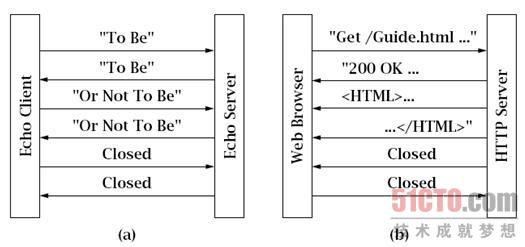
\includegraphics[scale=.8]{img/04.01.jpg}
		\caption{回显协议(a)与HTTP协议的终止(b)}
		\label{fig:echo.pt.and.http.end}
	\end{figure}

	Echo Client:回显客户端;Echo Server:回显服务器;Closed:关闭;Web Browser:网络浏览器;HTTP Server:HTTP服务器;Closed:关闭 

	实际上,客户端的关闭表示通信已经完成。HTTP协议也是一样的原理,只是它的通信终止发起者是服务器。 

	下面考虑另一种协议。假设你需要一个压缩服务器,将接收到的字节流压缩后,发回给客户端。这种情况下应该由哪一端来关闭连接呢?由于从客户端发来的字节流的长度是任意的,客户端需要关闭连接以通知服务器要压缩的字节流已经发送完毕。那么客户端应该什么时候调用close()方法呢?如果客户端在其发送完最后一个字节后立即调用套接字的close(),它将无法接收到压缩后数据的最后一些字节。或许客户端可以像回显协议那样,在接收完所有压缩后的数据才关闭连接。但不幸的是,这样一来服务器和客户端都不知道到底有多少数据要接收,因此这也不可行。我们需要一种方法来告诉连接的另一端"我已经发送完所有数据",同时还要保持接收数据的能力。 

	幸运的是套接字提供了一种实现这个功能的方法。Socket类的shutdownInput()和shutdownOutput()方法能够将输入输出流相互独立地关闭。调用shutdownInput()后,套接字的输入流将无法使用。任何没有发送的数据都将毫无提示地被丢弃,任何想从套接字的输入流读取数据的操作都将返回-1。当Socket调用shutdownOutput() 方法后,套接字的输出流将无法再发送数据,任何尝试向输出流写数据的操作都将抛出一个IOException异常。在调用shutdownOutput()之前写出的数据可能能够被远程套接字读取,之后,在远程套接字输入流上的读操作将返回-1。应用程序调用shutdownOutput()后还能继续从套接字读取数据,类似的,在调用shutdownInput()后也能够继续写数据。 

	在压缩协议中(见图4.2),客户端向服务器发送待压缩的字节,发送完成后调用shutdownOutput()关闭输出流,并从服务器读取压缩后的字节流。服务器反复地获取未压缩的数据,并将压缩后的数据发回给客户端,直到客户端执行了停机操作,导致服务器的read操作返回-1,这表示数据流的结束。然后服务器关闭连接并退出。 

	\begin{figure}[htbp]%位置选项
		\centering
		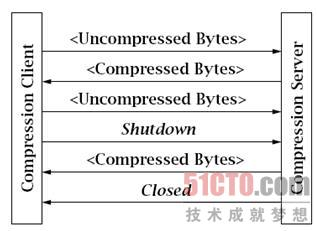
\includegraphics[scale=.8]{img/04.02.jpg}
		\caption{压缩协议终止}
		\label{fig:copose.pot.end}
	\end{figure}

	Compression Client:压缩客户端;Compression Server:压缩服务器;

	Uncompressed Bytes:未压缩字节;Compressed Bytes:已压缩字节;

	Shutdown:停机;Closed:关闭 

	在客户端调用了shutdownOutput之后,它还要从服务器读取剩余的已经压缩的字节。 

	下面的压缩客户端示例程序,CompressClient.java,实现了压缩协议的客户端。程序从命令行中指定的文件读取未压缩字节,然后将压缩后的字节写入一个新的文件。设未压缩文件名是"data",压缩后文件名是"data.gz"。注意,这个程序只适用于处理小文件,对于大文件来说其存在一个缺陷将导致死锁。(我们将在第6.2节讨论并改正这个缺陷。) 

	\lstinputlisting[language=Java,firstline=1]{src/ch04/CompressClient.java}

	1.应用程序设置和参数解析:

	2.创建套接字和打开文件:

	3.调用sendBytes()方法传输字节:

	4.接收压缩后的数据流:

	while循环反复接收压缩后的数据流并将字节写入输出文件,直到read()方法返回-1表示数据流的结束。 

	5.关闭套接字和文件流:

	6.sendBytes():

	给定一个连接到压缩服务器的套接字和一个文件输入流,从文件中读取所有未压缩的字节,并将其写入套接字的输出流。 

	获取套接字输出流:

	向压缩服务器发送未压缩字节:

	while循环从输入流读(在这个例子中是从一个文件)取数据并反复将字节发送到套接字的输出流,直到read()方法返回-1表示到达文件结尾。每一次写操作由打印到控制台的"W"指示。 

	关闭套接字输出流:

	在读取和发送完输入文件的所有字节后,关闭输出流,以通知服务器客户端已经完成了数据发送。close操作将导致服务器端的read()方法返回-1。 

	我们简单地为多线程的服务器构架写了一个协议,来实现压缩服务器。我们的协议实现,CompressProtocol.java,使用GZIP压缩算法实现了服务器端的压缩协议。服务器从客户端接收未压缩的字节,并将其写入GZIPOutputStream,它对套接字的输出流进行了包装。 

	\lstinputlisting[language=Java,firstline=1]{src/ch04/CompressProtocol.java}

	1.变量和构造函数:

	2.handleCompressClient():

	给定一个连接到压缩客户端的套接字,从客户端读取未压缩字节并将压缩后的字节写回客户端。 

	获取套接字I/O流:

	套接字的输出流包装在一个GZIPOutputStream中。写向这个流的字节序列将由GZIP算法对其进行压缩,然后再写入底层的输出流。 

	读取未压缩字节和写压缩后的字节:

	while循环从套接字输入流读取数据,并写入GZIPOutputStream,再由它将压缩后的数据写入套接字的输出流,直到接收到流结束标记。 

	刷新和关闭:

	在关闭GZIPOutputStream之前需要刷新提交可能被压缩算法缓存的字节。 

	run()方法:

	run()方法只是简单地对handleCompressClient()方法进行调用。 

	为了使用这个协议,我们对TCPEchoServerExecutor.java进行了简单的修改,创建了一个CompressProtocol实例来替代EchoProtocol实例: 

	\lstinputlisting[language=Java,firstline=147,lastline=147]{src/ch04/ThreadExample.txt}

\section{Applets} 

	Applet可以通过TCP/IP套接字在网络上进行通信,不过对于它们如何通信以及可以与谁通信有一些限制。如果没有这些限制,可信任的浏览器就可能执行有害的applet程序,例如,可能会发送欺骗邮件,或在用户使用浏览器时试图攻击其他系统,等等。这些安全性限制是由Java的安全管理器强制实施的,如果applet违法了这些限制,则将抛出SecurityException异常。通常,浏览器只允许applet与自身所在的宿主主机进行通信。这就意味着applet限制为只能与在宿主主机上执行的应用程序通信,通常是创建该applet的Web服务器。有关applet编程的安全性限制列表不属于本书的讨论范围,不过这也没多大价值,因为如果使用浏览器的用户允许的话,其默认的安全限制也可以改变。 

	假设现在需要实现一个允许用户在浏览器中输入和保存笔记的applet。由于浏览器的安全性限制阻止了applet直接向本地文件系统保存数据,因此要使用有别于本地磁盘输入输出的其他方法来保存笔记。FileClientApplet.java(见本书网站)实现了一个applet,它允许用户在一个编辑窗口中输入文本,点击"保存"按钮后,通过网络将文本复制到一个服务器上(运行在5000端口)。服务器,TCPFileServer.java(见本书网站),再将数据保存到一个文件中。它需要一个端口号(使用与applet对应的5000端口)和文件名作为参数。该服务器程序必须运行在向浏览器提供applet的Web服务器上。注意该服务器并没有任何applet特性。网页上的FileClientApplet.html文件演示了如果将applet整合到一个网页中。 

\section{结束} 

	本章中讨论了Java提供的一些访问套接字API高级特性的一些方法,以及如何使用多线程、执行器等内置功能来进行套接字编程。另外,Java还提供了一些机制(在这里没有作讨论),在TCP和UDP协议上层进行操作,并隐藏了协议开发的复杂性。例如,Java远程方法调用(Remote Method Invocation ,RMI)允许在不同主机上的Java对象相互调用彼此的方法,就像这些对象都驻留在本地一样。URL类以及其他相关类提供了一个开发Web程序的框架。还有不少标准的Java库,提供了很多各种令人惊奇的服务机制。这些机制不在本书的讨论范围之内,然而,我们建议你访问本书的网站,参考这些库的介绍并动手编写一些示例程序。 


